De XNOR\index{XNOR} geeft als \'e\'en van beide ingangen 1 is en de andere 0 een 0 op de uitgang.

\rowcolors{2}{gray!10}{gray!20}
\begin{tabular}{ |c|c|c| }
\hline
\rowcolor{gray!60}
	Input 1 & Input 2 & Output \\
	\hline
	0 & 0 & 1 \\
	\hline
	0 & 1 & 0 \\
	\hline
	1 & 0 & 0 \\
	\hline
	1 & 1 & 1 \\
	\hline
\end{tabular}

Het symbool voor de XNOR is weergegeven in figuur \ref{symbool:xnor}

\begin{figure}[h]
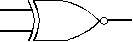
\includegraphics{xnor_symbool}
\centering
\caption{Symbool van een XNOR}
\label{symbool:xnor}
\end{figure}

Er zijn vele manieren om een XNOR te bouwen, er is dan ook geen circuit opgenomen. Zie Wikipedia voor mogelijke oplossingen.

